\documentclass[tikz,border=10pt]{standalone}
\usepackage{tikz}
\usetikzlibrary{calc}

\begin{document}

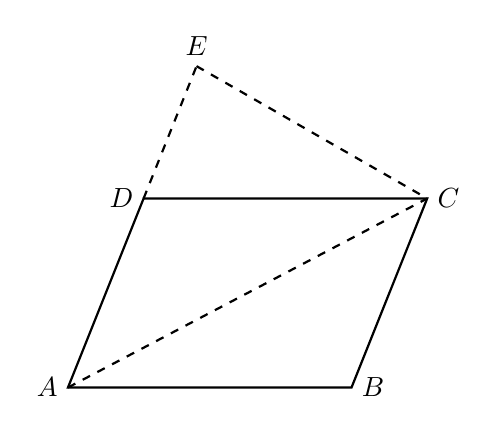
\begin{tikzpicture}[>=stealth, thick, scale=1.2]
    % 1. 定义核心顶点坐标 (基于平行四边形比例)
    \coordinate (A) at (0,0);
    \coordinate (B) at (3,0);
    \coordinate (D) at (0.8, 2);
    % 利用向量加法计算 C 点坐标，确保 ABCD 是平行四边形 (C = B + D - A)
    \coordinate (C) at ($(B)+(D)-(A)$);
    
    % 2. 定义辅助点 E (延长 AD 得到的点)
    % 这里设定 E 在 AD 的延长线上，距离 D 约 1.5 单位
    \coordinate (E) at ($(A)!1.7!(D)$);

    % 3. 绘制实线部分 (平行四边形主体)
    \draw (A) -- (B) -- (C) -- (D) -- cycle;

    % 4. 绘制虚线部分 (辅助线)
    \draw [dashed] (A) -- (C);      % 对角线 AC
    \draw [dashed] (D) -- (E);      % 延长线 DE
    \draw [dashed] (E) -- (C);      % 连接线 EC

    % 5. 标注顶点标签
    % anchor 调整标签位置，确保不遮挡线条
    \node [left]  at (A) {$A$};
    \node [right] at (B) {$B$};
    \node [right] at (C) {$C$};
    \node [left]  at (D) {$D$};
    \node [above] at (E) {$E$};

    % 6. (可选) 如果需要标注点，可以取消下行注释
    % \foreach \p in {A,B,C,D,E} \fill (\p) circle (1.5pt);

\end{tikzpicture}

\end{document}